	\chapter{ReLUSyn}
% To automate the FDI attacks, we follow a three-step approach.
%1. We first abstract the CPS DNN in a generalizable format developed by Dutta et al. \cite{10.1007/978-3-319-99429-1_11} that allows us to represent a trained network. 
%2. Using the trained network values we pass it through the MILP modeling that we have constructed. 
%3. We then find the optimal FDI values for the network. 

%{Explain in detail these three steps and explain the mathematical modeling here}
Our goal is to automate the attack synthesis for complex systems such as CPS that can handle the two challenges C1 and C2. This section illustrates how \tool helps achieve these goals by providing an approach for building automated attack synthesizers. We start with the illustration of attack synthesis workflow \ref{section:overview}, followed by an example of how to use \tool with a continuation of our motivating example, APS \ref{section:attacks}. In the next section, we describe the modeling of the cost function for conducting the attacks and how we were able to find the critical inputs \ref{section:costfunction}. %We end the section with a discussion of the limitations \ref{section:limitations}. 

\begin{figure}
	\centering
	\includegraphics[scale=0.1]{"Images/Methodology"}
	\caption[Methodology]{The rounded boxes depict the information provided by the users and the sharp corners is the information provided by us that integrates the first layer into the solver layer.}
	\label{fig:methodology-2}
\end{figure}



\subsection{Overview}
\label{section:overview}
%This section introduces the different layers and how the framework is designed. It talks about how MILP allows us to model the DNN. Where is the cost function placed? What happens when a user enters an infeasible model. 

%This para talks about the first layer from out figure, where the user provides the DNN values in form of the weights and the bias. Also, the reason we expect weights and bias is coz its a trained model for deployment. 
Figure 4 shows the \tool synthesizer stack. With \tool, developers/users can synthesize attacks for different domains of CPS built using DNNs. They provide the weights and bias of the trained DNN for the CPS. \tool will automatically infer the critical inputs and the perturbations to conduct \attack.
%\tool is not built to train secure models but in fact, it is used to find \attack in a trained model. %\tool provides an interface to provide the DNN in a simplified way.

%This paragraph is for explaining the cost function and the MILP modeling layer in layer 2 of our framework.  
The MILP modeling converts the DNN into linear constraints that are comprehensible for MILP solvers. Different cost functions can be modeled to integrate with the framework to generate different types of attacks. These cost functions guide the model to minimize and maximize \cite{Williams2013} perturbations. %We leverage the MILP capabilities to generate inputs that cause FDI.

%This explains the final layer which after taking in the MILP modeling and the cost function pass it through an optimizer which in this case we use is the gurobi optimizer. 
After the cost function and the DNN model have been defined we run it through the state-of-the-art backed solver Gurobi \cite{gurobi} that solves and returns optimal solutions if they exist. Otherwise, it returns an infeasible model to show the non-existence of ripples.

%Conclusion for the overview
In this section, we explain how \tool tackles the challenges we have described in the previous sections. %Our methodology focuses on designing an appropriate technique for our use case that is the attack synthesis; this includes finding the critical inputs and the appropriate perturbations. 
% modeling cost functions that provide that can be mapped back to the real system and, finally, how we dealt with state-space explosions.

%Finally, we emphasize two benefits of \tool. First, it allows the user (attacker in this case) to use the tool as a black box for producing FDI attacks by making the process automated. The attacker needs to just produce the parameters for the network that she is trying to attack. Given the parameters, \tool generates the appropriate FDI attacks. %There is currently no other tool/system that allows the attackers to attack this easily on DNN based systems. They require multiple attempts before they can successfully do an attack. Second, the technique ensures the production of results if they exist since we model the constraints in a way that utilizes Gurobi's power of optimization. 



\subsection{Building the model}
\label{section:attacks}
%This section focuses on how we build the model using MILP and some background insights about DNN along with that. 
\tool comes with automated attack synthesizers for Artificial Pancreas System, Aircraft Collision Avoidance systems ACAS Xu and Horizontal CAS. %Writing a new attack synthesizer into \tool boils down to defining the attack model as a function that can be easily plugged in our framework.
As an example, we use a toy Artificial pancreas system (toyAPS) and then explain APS. A toyAPS as shown in Figure 5 consists of two sensor inputs that predict the amount of insulin as the output at some time $t$. 
\begin{figure}
	\centering
	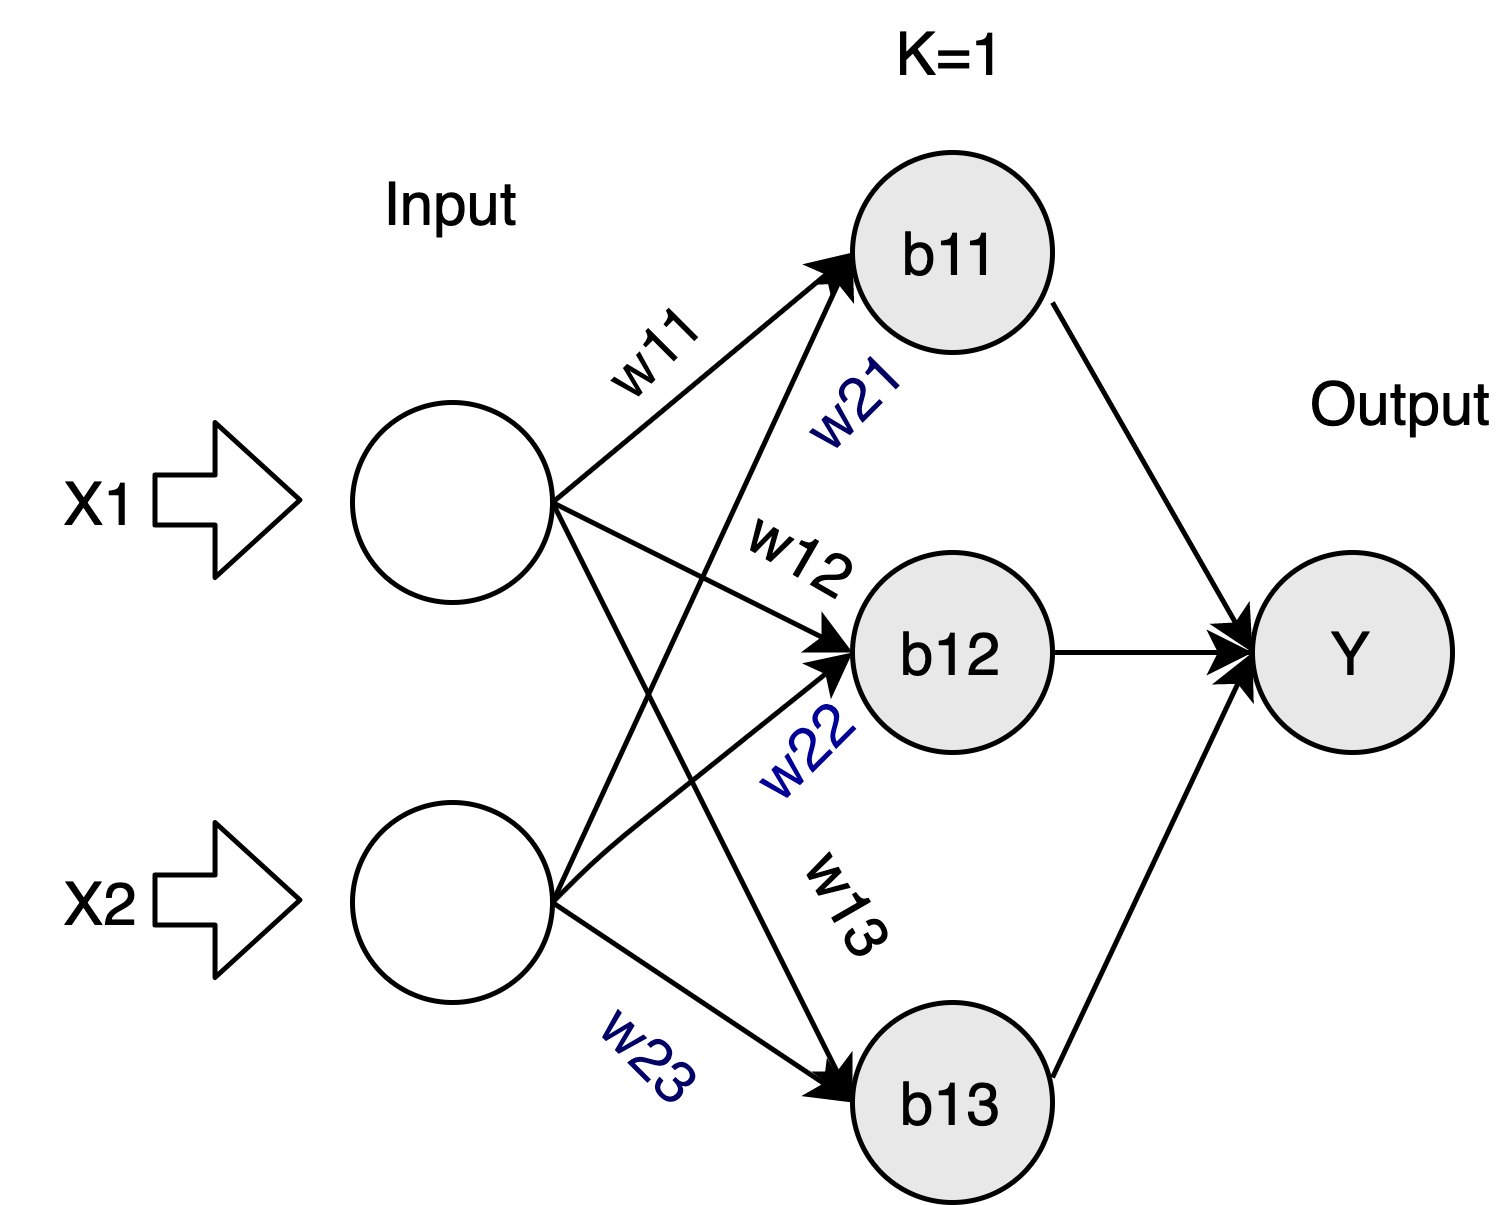
\includegraphics[width=0.7\linewidth]{Images/ToyAPS}
	\caption[A ToyAPS]{A ToyAPS that takes in two inputs which we consider as the sensor values from the human. It predicts the amount of insulin to be injected at some time based on the sensor inputs.}
	\label{fig:toyaps}
\end{figure}


\begin{algorithm}
	%\DontPrintSemicolon % Some LaTeX compilers require you to use \dontprintsemicolon    instead
	\KwIn{ weight, bias, num\_layers, num\_neurons}
	\KwOut{input, layer\_output, ReLU\_output}
	Take the weight, bias, number of layers and number of neurons per layer. \\
	
	\textbf{Model}, \linebreak
	%\renewcommand{\labelenumi}{(\Roman{enumi})}
	%\begin{enumerate}[noitemsep,nolistsep]
	%\item
	(I) For every  layer,  $expr = input * weight + bias$
	\linebreak 
	defining the linear expression
	\linebreak
	$layer\_output = expr$
	\linebreak
	%\item 
	(II) Define the non-linear activation function 
	\linebreak 
	\qquad Constraint: $ReLU(x) = max (0,x)$
	\linebreak
	(III) Adding non-linearity to every layer,
	\linebreak
	Constraints: $ReLU\_output = ReLU(0, layer\_output)$\\, 
	Repeat Step 2 until all layers are modeled 
	\linebreak
	$num\_layers < = 0$   $ \&\& $ 
	$ num\_neurons < = 0 $.
	
	\caption{Modeling neural network in MILP}
	\label{algo:b}
\end{algorithm}


The system can be represented as a MILP model through pseudo-code in Algorithm 1. This converts the neural network structure into a set of linear equations that can be mapped directly into a back-end MILP solver (we use Gurobi). %For our work we model our networks in Gurobi. 

\begin{align*}
Y &=  ReLU(Wx + b) ...... (4)
%Y &= ReLU(w_{11} x_1 + b_{11}  + w_{12} x_1 + b_{12} + w_{13} x_1 + b_{11}   )   \\
\end{align*}
The above equation represents the toyAPS. We convert the equations above into a MILP model as shown in Algorithm 1. Every layer is initially modeled as a linear equation. The activation function is represented as piecewise linear. Our approach will work for any representation of a piece-wise linear function. However, in our work we specifically focus on ReLU as explained in the problem formulation section. 
\subsection{Modeling cost functions for attacks}
\label{section:costfunction}
%Why is modeling cost function important
After representing the pictorial representation of a network as shown in Figure 5 to Algorithm 1, the next step is to model the cost or objective function. The cost function is what decides on the smallest perturbations of the inputs for generating a ripple. 

In our toyAPS we have two inputs $x_1$ and $x_2$ that map to an output $y$. To conduct \attack the goal is to change the inputs in a way that the alarms are not triggered and yet it leads to an output change. These small changes lead the system to end up in a bad state eventually. In toyAPS, every small increase is a bad consequence of the system. Since the output determines the amount of insulin to be injected inside the body, small increases in the output can cause the diabetic patient harm \cite{ZHANG2019403} and can lead to cancer. 
Therefore in toyAPS the attacker's goal is to change the output to $y'$, where $y' = y + a$. $a$ is some constant. %She needs to find the deviations in the input that would help her to change the outputs. 
However, the catch here is that the inputs perturbations should be very small such that the new input now provides her the output $y'$.  The reason she wants the input perturbations to be small is that there are accompanying neural networks that determine the upper and lower bounds for inputs and outputs at every stage. The reason for these accompanying networks is to ensure the patients' safety as explained in Section IV.%Hence, we have to minimize the perturbations. 
%This paragraph is explaining the subtlety of how we model our inputs for minimizing the perturbations. 
%We are hence minimizing the perturbations and not the inputs directly. Since minimizing the inputs directly will provide us with the smallest set of inputs that cause a deviation in the output. However, we want the smallest possible perturbations from the original image that change the output by the amount we want it to deviate. To find the smallest perturbations, we introduce a new variable delta for every input in the system. The new input is the addition of the original value and the minimized delta that ReLUSyn produces. 

Algorithm 1 describes the process of modeling a neural network in a MILP format. It does not consist of the cost function since the function will be different for systems depending on what the attacker wants to minimize and/or maximize. We model the objective function by introducing a new variable called $input\_delta$. Hence now the equation (1) in this section can be redefined as:

\begin{align}
Y &=  ReLU(W(x + \bigtriangleup  x ) + b) ...... (5)
\end{align}

%The new cost modeling adds one layer of extension to our previous algorithm which is the objective function. Modeling any DNN can be done in the way presented in Algorithm 1 so long the activation function can be described as piecewise linear. 
%\smi{for MILP, this is only true if the activation function is piecewise linear}.
Algorithm 2 shows how to include the cost functions for different attacks as a part of the MILP model. The cost function can be changed based on the attack requirements. 
\begin{algorithm}
	%\DontPrintSemicolon % Some LaTeX compilers require you to use \dontprintsemicolon    instead
	\KwIn{ weight, bias, num\_layers, num\_neurons}
	\KwOut{input, input\_delta layer\_output, ReLU\_output,}
	Take the weight, bias, number of layers and number of neurons per layer. \\
	
	\textbf{Model}, \linebreak
	%\renewcommand{\labelenumi}{(\Roman{enumi})}
	%\begin{enumerate}[noitemsep,nolistsep]
	%\item
	(I) For every  layer,  $expr = input * weight + bias$
	\linebreak 
	defining the linear expression
	\linebreak
	$layer\_output = expr$
	\linebreak
	%\item 
	(II) Define the non-linear activation function 
	\linebreak 
	\qquad Constraint: $ReLU(x) = max (0,x)$
	\linebreak
	(III) Adding non-linearity to every layer,
	\linebreak
	Constraints: $ReLU\_output = ReLU(0, layer\_output)$\\, 
	Repeat Step 2 until all layers are modeled 
	\linebreak
	$num\_layers < = 0$   $ \&\& $ 
	$ num\_neurons < = 0 $.\\
	
	\textbf{Cost/Attack Function} \linebreak
	$Minimize $  $input\_delta$
	\caption{Modeling neural network in MILP}
	\label{algo:b}
\end{algorithm}

If there are two inputs as in our toyAPS, we can either try to minimize the delta values for both the inputs or only one of the inputs. The reason it is important to understand this is because, in general, APS, there are inputs that come from two different sensors as explained in the motivating example section. %The first sensor is attached to the back of the patient that captured the blood-glucose levels of the patient and the second input is from the insulin pump to get the measure of the insulin level in the pump.
The attacker might want to make changes to only one of the sensor readings. Hence, considering different scenarios, we can minimize the values depending on which input we are interested in conducting an FDI attack. 

\subsection{Finding critical inputs}
In our running example of APS, in reality, there are 74 inputs collected from two sensors every five minutes. The goal of the attacker is to locate the critical inputs such that they can conduct FDI at the right time. To do so, as described in the previous two sections, the tool can be used to chose the index of inputs to be perturbed. 

If the attacker wants to locate one input that on perturbing by the smallest amounts can lead to the output change, they can specifically choose those inputs for conducting \attack.

%Depending on the attack model of the attacker, they can choose input(s) they are interested in finding the minimum perturbations for. We have implemented a framework that allows the users to pass the input index for inputs to be perturbed as a parameter. We will show this in the Evaluation section in more detail. 
\label{section:cost function}
\subsection{Synthesizing attacks}
The final part is synthesizing the inputs that can be used to conduct \attack without triggering any alarms in the system. To do so we introduce the final constraints that put lower and upper bounds on the output of the networks. This is important for the optimization to return useful results. The reason the optimization approach wins here is that if we provide the proper constraints it gives us results in less than a second per attack. This precise modeling is the secret sauce that scales up our technique significantly and provides us \attack based on the scenario. Due to the proper ranges, the state space is handles well by our technique and does not result in blowups. 
%\aarti{Should I add more here and also the algorithm for the synthesizing attack aspect?}              

